\subsection{Fundamentals of real-time technologies}

Before exploring various frameworks and strategies for implementing real-time communication in web applications, it's essential to establish a foundational understanding of real-time technologies. This understanding ensures that a developer is ready to navigate the complexities of real-time communication effectively. By gaining insight into these fundamental concepts, one can make informed decisions, troubleshoot issues, and optimise performance when integrating real-time features into applications.

\textbf{Methodologies:} Literature review, case studies

\subsubsection{Scope of this research}

It's crucial to establish the scope of this research, which primarily focuses on real-time communication within web applications. While real-time communication incorporates various forms, such as MQTT for IoT communication and SignalR for .NET applications, this study specifically centres on its implementation within web-based environments. By narrowing the scope to web applications, we can delve deeply into the unique challenges, requirements, and solutions associated with real-time communication in this context.

There are lots of technologies \cite{alby-ws-alt} that can be used to achieve real-time communication, keep in mind these are not yet categorised for a certain use case.

\begin{enumerate}
  \item WebSocket
  \item WebTransport
  \item Server-Sent Events
  \item WebRTC
  \item gRPC
  \item GraphQL Subscriptions
\end{enumerate}

\pagebreak

\subsubsection{Focused technologies}

This study will already narrow down our focus to WebSockets, WebTransport, and Server-Sent Events, delving into their respective concepts. The decision to focus on these technologies is based on several considerations. First of all due to their widespread adoption and relevance in typical web applications. Additionally, they offer a straightforward implementation and integration processes, making them suitable for a general research scope.

WebSockets, known for their bidirectional communication capabilities, are widely supported across browsers and standardised through the RFC 6455 specification. Similarly, Server-Sent Events offer a simple and efficient method for server-to-client communication, particularly suited for scenarios where one-way data flow suffices.

WebTransport, while still emerging, shows promise as a next-generation transport protocol for the web, offering improved performance and efficiency over the TCP-based WebSocket protocol.

Conversely, exclusion of gRPC, WebRTC and GraphQL from the research focus is due to their specialised use cases and setup requirements, which may not align with the general scope of this study. gRPC is certainly well-suited for applications that already utilise the Remote Procedure Call (RPC) paradigm. However, for web applications focusing on real-time collaborative features, the complexity of implementing and configuring gRPC may outweigh its benefits, especially when compared to more straightforward alternatives like WebSockets or Server-Sent Events.

Similarly, WebRTC, while suitable for peer-to-peer streaming of video and voice, is not primarily designed for collaborative features, which are the primary focus of this research.

The reasoning behind excluding GraphQL subscriptions is primarily due to its dependency on a GraphQL API, which may limit its applicability to a broader range of web applications. GraphQL also uses WebSockets under the hood so it's better to focus on more general-purpose solutions like WebSockets or Server-Sent Events.

It's important to note that this reasoning can be applied to various other technologies not listed as well. Many specialised or niche technologies may have dependencies or requirements that make them less suitable for general research or widely applicable use cases. By focusing on technologies like WebSockets, WebTransport, and Server-Sent Events, this research aims to provide insights and recommendations that are relevant and accessible to a broader audience of web developers.

\subsubsection{Evolution of real-time communication}

Real-time communication has undergone a remarkable evolution, paving the way for modern technologies like WebSockets and Server-Sent Events (SSE) to revolutionise the way data is transmitted over the web. Looking into the history of these innovations unveils a fascinating narrative of ingenuity and technological advancement.

In the early days of the internet, traditional HTTP-based approaches, such as polling and long polling, were used to simulate real-time updates. However, these methods were inefficient and abused the HTTP protocol resulting in unnecessary network traffic and latency issues. Additionally, techniques like Forever Frames attempted to maintain persistent connections but were limited in scope and compatibility. \cite{telerik-rtc}

\begin{enumerate}
  \item Polling: Clients would repeatedly send requests to the server to check for updates, resulting in inefficient network traffic.
  \item Long Polling: Clients would send a request to the server, which would hold the connection open until new data was available or a timeout occurred, reducing the number of requests but still having limitations.
  \item Forever Frames: A technique used in older versions of Internet Explorer, Forever Frames involved creating an invisible iframe that continuously loaded a script from the server to maintain an open connection for data updates.
\end{enumerate}

Recognizing the limitations of traditional HTTP-based communication, developers began exploring new avenues to facilitate real-time interactions on the web. AJAX (Asynchronous JavaScript and XML) introduced asynchronous data exchange, allowing web pages to update dynamically without full page reloads. Meanwhile, Comet-based techniques enabled server push and long-lived connections. \cite{alby-ws}

\textbf{Modern solutions}

The breakthrough in real-time web communication came with the introduction of the WebSocket protocol. Conceived as a standard for bidirectional, full-duplex communication, WebSocket revolutionised the way data is exchanged between clients and servers. By establishing persistent connections over a single TCP connection, WebSocket overcame the limitations of traditional HTTP-based approaches and provided a more efficient mechanism for real-time data transfer. \cite{alby-ws}

In 2011, the WebSocket protocol was standardised by the Internet Engineering Task Force (IETF) through RFC 6455 \cite{mdn-ws}. This standardisation marked a significant milestone in the evolution of real-time web communication, paving the way for widespread adoption and integration into web applications. Today, WebSocket is widely supported across browsers and serves as the foundation for a wide range of real-time applications, from chat applications to collaborative document editing platforms.

In addition to WebSocket, Server-Sent Events (SSE) also play a crucial role in facilitating real-time communication on the web. Unlike WebSocket, which enables bidirectional communication, SSE enables servers to push updates to clients over a single, long-lived HTTP connection \cite{mdn-sse}. While SSE may not offer the same level of interactivity as WebSocket, it is well-suited for scenarios where one-way data flow suffices, such as streaming updates, live feeds, and real-time notifications.

\textbf{Emeging solutions}

While WebSockets have become a foundational technologie for real-time communication on the web, WebTransport aims to enhance web applications further. Offering a solutions to the head-of-line blocking issue and better performance, WebTransport is still in its experimental stage and not yet widely adopted \cite{mdn-wt}. Despite this, the evolution of real-time web communication continues to be driven by technological advancements and developer needs.

\subsubsection{WebSocket fundamentals}

WebSocket is a communication protocol that provides full-duplex channels over a single, persistent connection. Full-duplex means this protocol allows data to be transmitted in both directions, simultaneously. In the context of WebSockets this means that both client and server can send and receive data without having to wait for one another.

It's designed to provide a responsive user experience by maintaining that open connection, unlike HTTP. Supported by its low latency, WebSockets ensure a genuine real-time experience. \cite{ws-rfc}

\textbf{High level overview}

\begin{enumerate}
  \item Opening a connection: \\ Opening handshake over HTTP request/response exchange between client and server.
  \item Data transfer: \\ Client and server exchange frames over a WebSocket connection, built on top of TCP.
  \item Closing a connection: \\ The connection can be terminated by either client or server by initiating a closing handshake.
\end{enumerate}

\begin{figure}[h]
  \caption{WebSocket connection diagram}
  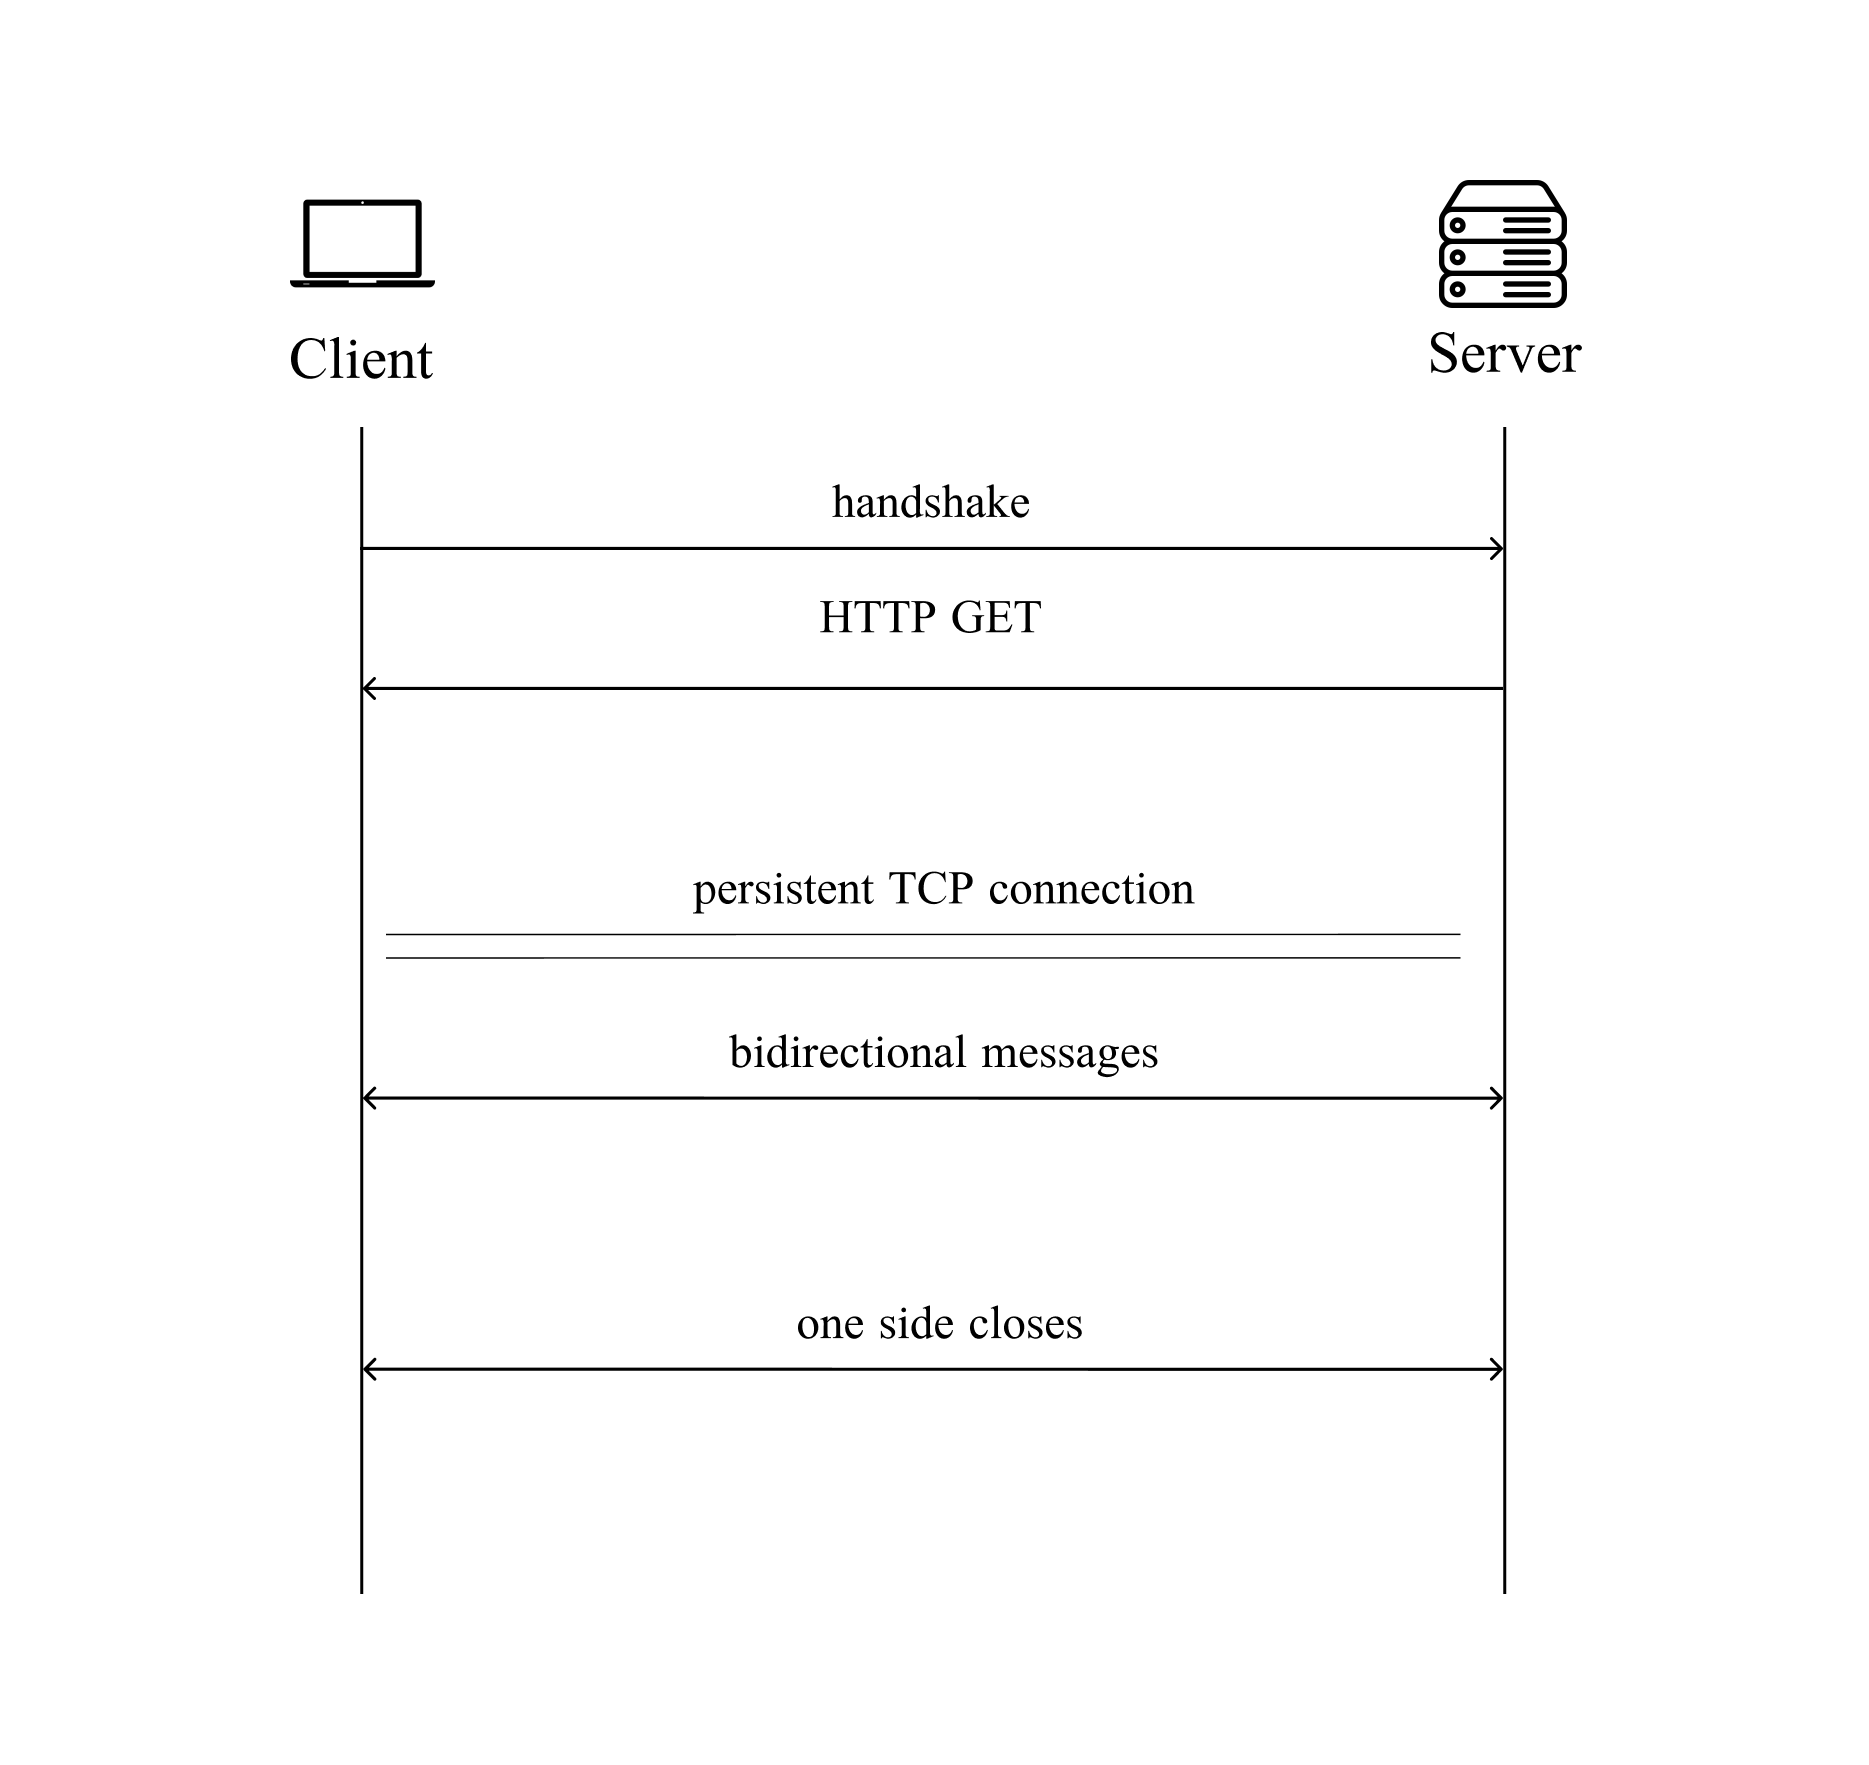
\includegraphics[width=0.8\linewidth]{websocket_diagram}
  \centering
\end{figure}

\textbf{Opening handshake}

The opening of a connection is intended to be compatible with HTTP-based architectures so that a single port can be used. This makes it possible that both HTTP clients and WebSocket clients can talk to the same server on the same port. \cite{ws-rfc}

The HTTP request in request-line format and in compliance with HTTP:
\begin{lstlisting}[caption=WebSocket opening handshake HTTP GET Upgrade request, style=nohighlight]
  GET /request-uri HTTP/1.1 
  Host: server.example.com 
  Upgrade: websocket Connection: Upgrade 
  Sec-WebSocket-Key: dGhlIHNhbXBsZSBub25jZQ== 
  Origin: http://example.com 
  Sec-WebSocket-Protocol: chat, superchat 
  Sec-WebSocket-Version: 13  
\end{lstlisting}

\begin{itemize}
  \item request-uri:  to identify the endpoint to allow multiple WebSockets to be served by a single server.
  \item Sec-Websocket-Protocol: an additional header to select a subprotocol layered over the WebSocket protocol.
\end{itemize}

The server needs to prove to the client that it received the request:
\begin{lstlisting}[caption=WebSocket opening handshake server response, style=nohighlight]
  HTTP/1.1 101 Switching Protocols
  Upgrade: websocket
  Connection: Upgrade
  Sec-WebSocket-Accept: s3pPLMBiTxaQ9kYGzzhZRbK+xOo=
  Sec-WebSocket-Protocol: chat
\end{lstlisting}

\begin{itemize}
  \item Sec-Websocket-Accept: a key + GUID hashed and encoded to provide proof.
  \item 101: anything else than 101 means that the handshake was not completed.
\end{itemize}

\textbf{Data transfer}

After a successful handshake data transfer is possible in conceptual units referred to as messages. On the wire those messages are broken down into frames. It is important to note that the protocol does not correspond to a certain network layer (OSI - TCP/IP) like how for example IP operates on the network layer, this protocol is not directly tied to a way packets are framed at the network layer. The message may be split into pieces by a router, the pieces can be mixed with other messages over different routes and later be grouped back together. \cite{ws-rfc}

\begin{enumerate}
  \item Spltting into frames:
        \begin{enumerate}
          \item[a.] Split into frames, the basic unit of data in the WebSocket protocol.
          \item[b.] Frames can be send in any order and can be mixed with frames from other messages.
          \item[c.] This optimises the use of available paths and accommodates different network conditions.
        \end{enumerate}
  \item The frames are reassembled into a complete message at the receiving end by position information contained in each frame
\end{enumerate}

\begin{lstlisting}[caption=Frame format, style=nohighlight]
 0                   1                   2                   3
 0 1 2 3 4 5 6 7 8 9 0 1 2 3 4 5 6 7 8 9 0 1 2 3 4 5 6 7 8 9 0 1
+-+-+-+-+-------+-+-------------+-------------------------------+
|F|R|R|R| opcode|M| Payload len |    Extended payload length    |
|I|S|S|S|  (4)  |A|     (7)     |             (16/64)           |
|N|V|V|V|       |S|             |   (if payload len==126/127)   |
| |1|2|3|       |K|             |                               |
+-+-+-+-+-------+-+-------------+ - - - - - - - - - - - - - - - +
|     Extended payload length continued, if payload len == 127  |
+ - - - - - - - - - - - - - - - +-------------------------------+
|                               |Masking-key, if MASK set to 1  |
+-------------------------------+-------------------------------+
| Masking-key (continued)       |          Payload Data         |
+-------------------------------- - - - - - - - - - - - - - - - +
:                     Payload Data continued ...                :
+ - - - - - - - - - - - - - - - - - - - - - - - - - - - - - - - +
|                     Payload Data continued ...                |
+---------------------------------------------------------------+
\end{lstlisting}

\textbf{Closing handshake}

The closing handshake is initiated by either peer sending a control frame with data containing a specified control sequence. The other peer sends a control frame back and the first peer then closes the connection, knowing that no further data is coming.

The sequence is intended to be a complement to the TCP close sequence. The TCP close sequence is not reliable end-to-end as it can be lost or delayed. By sending a close frame and waiting for one in return no data will be lost.

WebSockets are designed to have minimal framing and expect metadata to be layered on top by the application, just as with TCP. WebSocket is a layer itself on top of TCP that adds web origin-based security, multiple devices on one port and a modified closing handshake.

The WebSocket protocol is an independent TCP-based protocol and its only connection to HTTP is its opening handshake interpreted by HTTP servers as an Upgrade request and that it also uses port 80 and 443 as default ports. \cite{ws-rfc}

\subsubsection{Server-Sent Events (SSE) fundamentals}

Server-Sent Events or simply referred to as SSE offer one-way data flow. This is suitable for unidirectional communications, such as a server to client notification. With SSE there is also a persistent connection but using the HTTP protocol so only the server can send data to the client at any time.

SSE is natively supported in browsers by using the EventSource interface, using this API consists of creating an EventSource object and registering an event listener. \cite{html-spec-sse}

\textbf{EventSource API}

The EventSource API uses an Interface Definition Language (IDL) to define the structure and behavior of the EventSource API in a formal specification. It outlines the methods, properties, and events that make up the EventSource interface, providing a standardized way for developers to understand and implement the API across different platforms and programming languages. \cite{html-spec-sse}

\begin{lstlisting}[caption=EventSource API IDL]
[Exposed=(Window,Worker)]
interface EventSource : EventTarget {
  constructor(
    USVString url,
    optional EventSourceInit eventSourceInitDict = {}
  );

  readonly attribute USVString url;
  readonly attribute boolean withCredentials;

  // ready state
  const unsigned short CONNECTING = 0;
  const unsigned short OPEN = 1;
  const unsigned short CLOSED = 2;
  readonly attribute unsigned short readyState;

  // networking
  attribute EventHandler onopen;
  attribute EventHandler onmessage;
  attribute EventHandler onerror;
  undefined close();
};

dictionary EventSourceInit {
  boolean withCredentials = false;
};
\end{lstlisting}

Because the concept of SSE is not a technologie by its self but a concept utilising HTTP, it is not a protocol like WebSockets, the IDL can be used to implement the API in any language or platform. Not only does it provide a blueprint to implement the API outside of the browser but it also let's developers understand and implement their own libraries or frameworks.

\subsubsection{WebTransport fundamentals}

WebTransport is a new protocol meant to replace the WebSocket protocol but is not widely supported yet. While this is changing quickly with recently added support in Chromium browsers beside the early support in Firefox, WebTransport is still in its early staging but is a promising upgrade from WebSocket.

WebTransport uses HTTP/3 built on the QUIC protocol that is using UDP instead of TCP. This fixes several issues around the classic TCP protocol on which HTTP and WebSocket are based. \cite{w3-wt}

\begin{enumerate}
  \item Head-of-line blocking: \\ HTTP/2 allows multiplexing, so a single connection can stream multiple resources at once. However, if a single resource fails, all other resources on that connection are held up until any missing packets are retransmitted. With QUIC, only the failing resource is affected.
  \item Faster: \\ QUIC outperforms TCP with built-in security features, fewer round trips and more efficient streams. This is especially advantageous on high-latency networks.
  \item Better network transitions: \\ QUIC uses a unique connection ID for packet delivery that allows downloads to resume seamlessly when switching between networks. In contrast, HTTP/2 relies on IP addresses.
\end{enumerate}

Choosing WebTransport at this stage may not be advisable for developers seeking immediate solutions due to its experimental nature and ongoing development. However, as WebTransport evolves and becomes more stable, it holds the potential to be a replacement or complement to existing real-time communication technologies like WebSocket and Server-Sent Events. Therefore, while it may not be the optimal choice for current development projects, monitoring the progress of WebTransport and understanding its capabilities can inform future decision-making and development strategies.

\subsubsection{Conclusion}

Real-time communication, which is necessary for implementing collaborative functionalities, is achieved through the use of protocols and technologies that enable efficient and responsive data transfer between clients and servers. WebSockets is the standard and most widely used technology for real-time communication on the web, providing a full-duplex communication channel over a single TCP connection. It is well-suited for real-time applications such as chat, gaming and mutliplayer collaboration tools. Other alternatives such as GraphQL Subscriptions, MQTT, gRPC and WebRTC are designed for specific use cases and may not be suitable for general-purpose real-time communication. However, for scenarios where only one-way communication from the server is needed, Server-Sent Events (SSE) suffices, providing a simpler alternative. Looking forward, while WebTransport holds promise for future advancements in real-time web communication, its full potential remains to be realised, marking it as a technology to watch as it matures.

To further understand the practical application of these technologies, see Apendix A: Case study Figma. By exploring Figma's innovative use of WebSockets to facilitate seamless collaboration, this study can gain valuable insights into how WebSocket work in practice.
